% LaTeX Template: Project Titlepage Modified (v 0.1) by rcx
%
% Original Source: http://www.howtotex.com
% Date: February 2014
% 
% This is a title page template which be used for articles & reports.
% 
% This is the modified version of the original Latex template from
% aforementioned website.

\documentclass[12pt]{article}
\usepackage[a4paper]{geometry}
\usepackage[myheadings]{fullpage}
\usepackage{fancyhdr}
\usepackage{lastpage}
\usepackage{graphicx, wrapfig, setspace, booktabs}
\usepackage[T1]{fontenc}
\usepackage[font=small, labelfont=bf]{caption}
\usepackage{fourier}
\usepackage[protrusion=true, expansion=true]{microtype}
\usepackage[english]{babel}
\usepackage{sectsty}
\usepackage{url, lipsum}
\usepackage{tgbonum}
\usepackage{hyperref}
\usepackage{xcolor}
\usepackage{enumerate}
\usepackage{listings}
\usepackage{lstautogobble}
\usepackage{subfigure}

\newcommand{\HRule}[1]{\rule{\linewidth}{#1}}
\onehalfspacing
\setcounter{tocdepth}{5}
\setcounter{secnumdepth}{5}



%-------------------------------------------------------------------------------
% HEADER & FOOTER
%-------------------------------------------------------------------------------
\pagestyle{fancy}
\fancyhf{}
\setlength\headheight{15pt}
\fancyhead[L]{Student ID: 10406141}
\fancyhead[R]{University of Manchester}
\fancyfoot[R]{Page \thepage\ of \pageref{LastPage}}
%-------------------------------------------------------------------------------
% TITLE PAGE
%-------------------------------------------------------------------------------

\begin{document}
{\fontfamily{cmr}\selectfont
\title{ \normalsize \textsc{}
		\\ [2.0cm]
		\HRule{0.5pt} \\
		\LARGE \textbf{\uppercase{Lab3B Report}
		\HRule{2pt} \\ [0.5cm]
		\normalsize \today \vspace*{5\baselineskip}}
		}

\date{}

\author{
		Wenchang Liu \\ 
		ID: 10406141 \\
		School of Computer Science }

\maketitle
\newpage
\tableofcontents
\newpage

%-------------------------------------------------------------------------------
% Section title formatting
\sectionfont{\scshape}
%-------------------------------------------------------------------------------

%-------------------------------------------------------------------------------
% BODY
%-------------------------------------------------------------------------------

\section{Ex1 Building a CFG}
\label{sec: ex1}
\begin{enumerate}[1.]
	\item Steel is an alloy.
    
    S -> NN VP .

    NP -> NN .

    VP -> VBZ NP.

    NP -> DT NN .

    NN -> Steel .

    VBZ -> is .

    DT -> an .

    NN -> alloy .
    
	\item Steel contains carbon.
    
    S -> NN VP .

    NP -> NN .

    VP -> VBZ NP .

    % NP -> NN .

    NN -> Steel .
    
    VBZ -> contains .
    
    NN -> carbon .

    \item We can combine them together.
    
    S -> NN VP .

    NP -> NN .

    VP -> VBZ NP .

    NP -> DT NN .

    NN -> Steel . NN -> alloy . NN -> carbon .

    VBZ -> is . VBZ -> contains.

    DT -> an .

\end{enumerate}

\newpage
\section{Ex2 Building a CFG in Prolog}
\label{sec: ex2}
\begin{enumerate}[1.]
    \item Translate the CFG grammar from the previous exercise into Prolog using difference lists.
        
    See the prolog file $cfg.pl$ in appendix A.
    \item Check if the grammar is able to recognise the two sentences.
        
    Yes.
    \item Generate all the sentences which can be recognised by this grammar.
    
    Query: s(X, []).
    
    X = [steel, is, steel] ;

    X = [steel, is, alloy] ;

    X = [steel, is, carbon] ;

    X = [steel, is, an, steel] ;

    X = [steel, is, an, alloy] ;

    X = [steel, is, an, carbon] ;

    X = [steel, contains, steel] ;

    X = [steel, contains, alloy] ;

    X = [steel, contains, carbon] ;

    X = [steel, contains, an, steel] ;

    X = [steel, contains, an, alloy] ;

    X = [steel, contains, an, carbon] ;

    X = [alloy, is, steel] ;

    X = [alloy, is, alloy] ;

    X = [alloy, is, carbon] ;

    X = [alloy, is, an, steel] ;

    X = [alloy, is, an, alloy] ;

    X = [alloy, is, an, carbon] ;

    X = [alloy, contains, steel] ;

    X = [alloy, contains, alloy] ;

    X = [alloy, contains, carbon] ;

    X = [alloy, contains, an, steel] ;

    X = [alloy, contains, an, alloy] ;

    X = [alloy, contains, an, carbon] ;

    X = [carbon, is, steel] ;

    X = [carbon, is, alloy] ;

    X = [carbon, is, carbon] ;
    
    X = [carbon, is, an, steel] ;
    
    X = [carbon, is, an, alloy] ;
    
    X = [carbon, is, an, carbon] ;
    
    X = [carbon, contains, steel] ;
    
    X = [carbon, contains, alloy] ;
    
    X = [carbon, contains, carbon] ;
    
    X = [carbon, contains, an, steel] ;
    
    X = [carbon, contains, an, alloy] ;
    
    X = [carbon, contains, an, carbon].
\end{enumerate}

\section{Ex3 DCGs}
\label{sec: ex3}
\begin{enumerate}[1.]
    \item Rephrase the previous grammar into a DCG.
    
    See prolog files $dcg.pl$ in appendix B.
    \item Check if you can recognise and generate the same sentences.
    
    Yes. It gets the same results as CFG.
\end{enumerate}

\section{Ex4 CCGs}
\label{sec: ex4}
\begin{enumerate}[1.]
    \item Create a CCG Grammar which recognises these sentences.  
    
    Steel: N

    is: (S$\backslash$N)/NP

    an: NP/N

    alloy: N

    contains: (S$\backslash$N)/N

    carbon: N

    Does: S/(S$\backslash$NP)/NP

    Ferrite: NP

    have: (S$\backslash$NP)/N

    high: N/N

    hardness: N

    Which: S/(S$\backslash$NP)/N

    material: N

    has: (S$\backslash$NP)/NP

    the: NP/N

    lowest: N/N

    tensile: N/N 

    strength: N
    \item Draw the derivation trees for each sentence.
    \begin{figure}[ht]
        \centering
        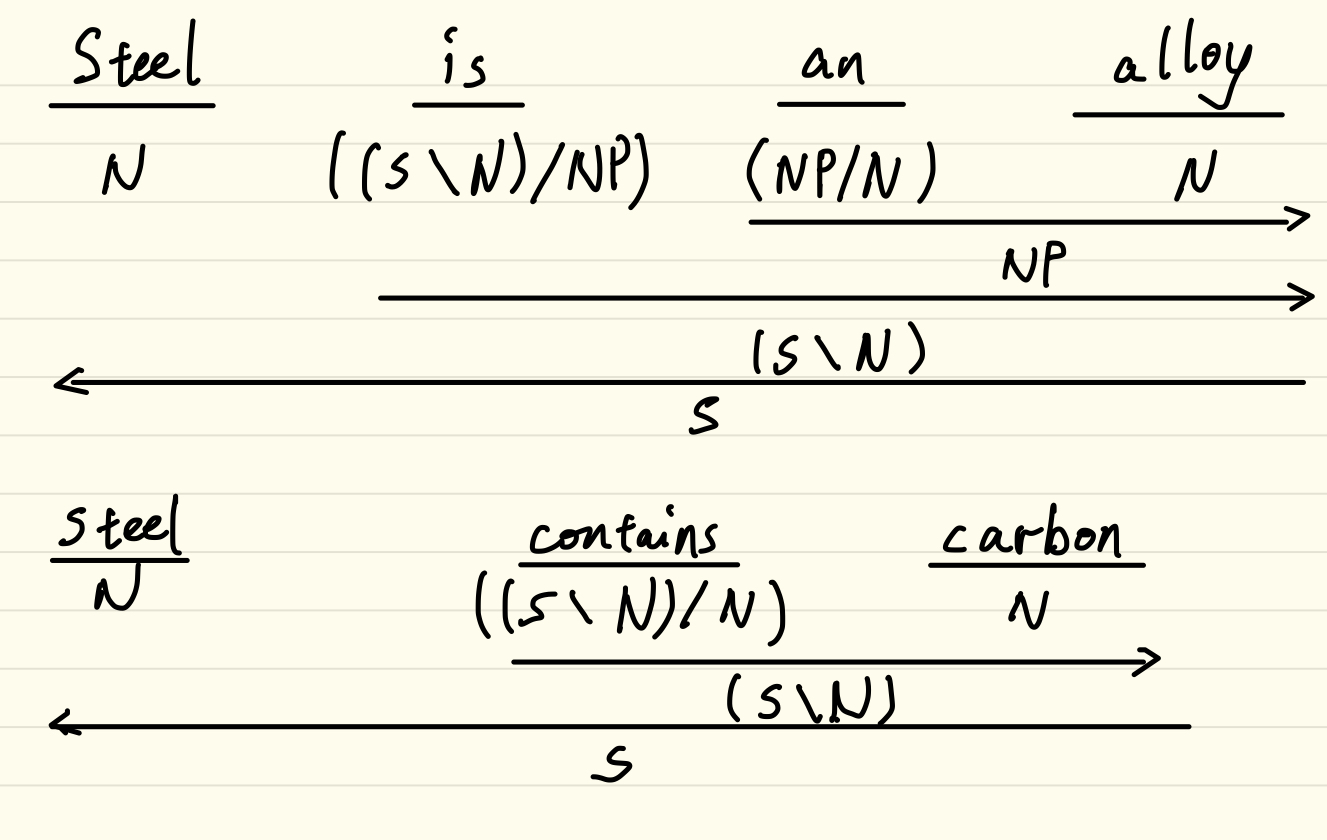
\includegraphics[scale=0.2]{figs/derTree1.jpg}
        \caption{derivation trees for statements}
        \label{label:derivation tree 1}
    \end{figure}
    \begin{figure}[ht]
        \centering
        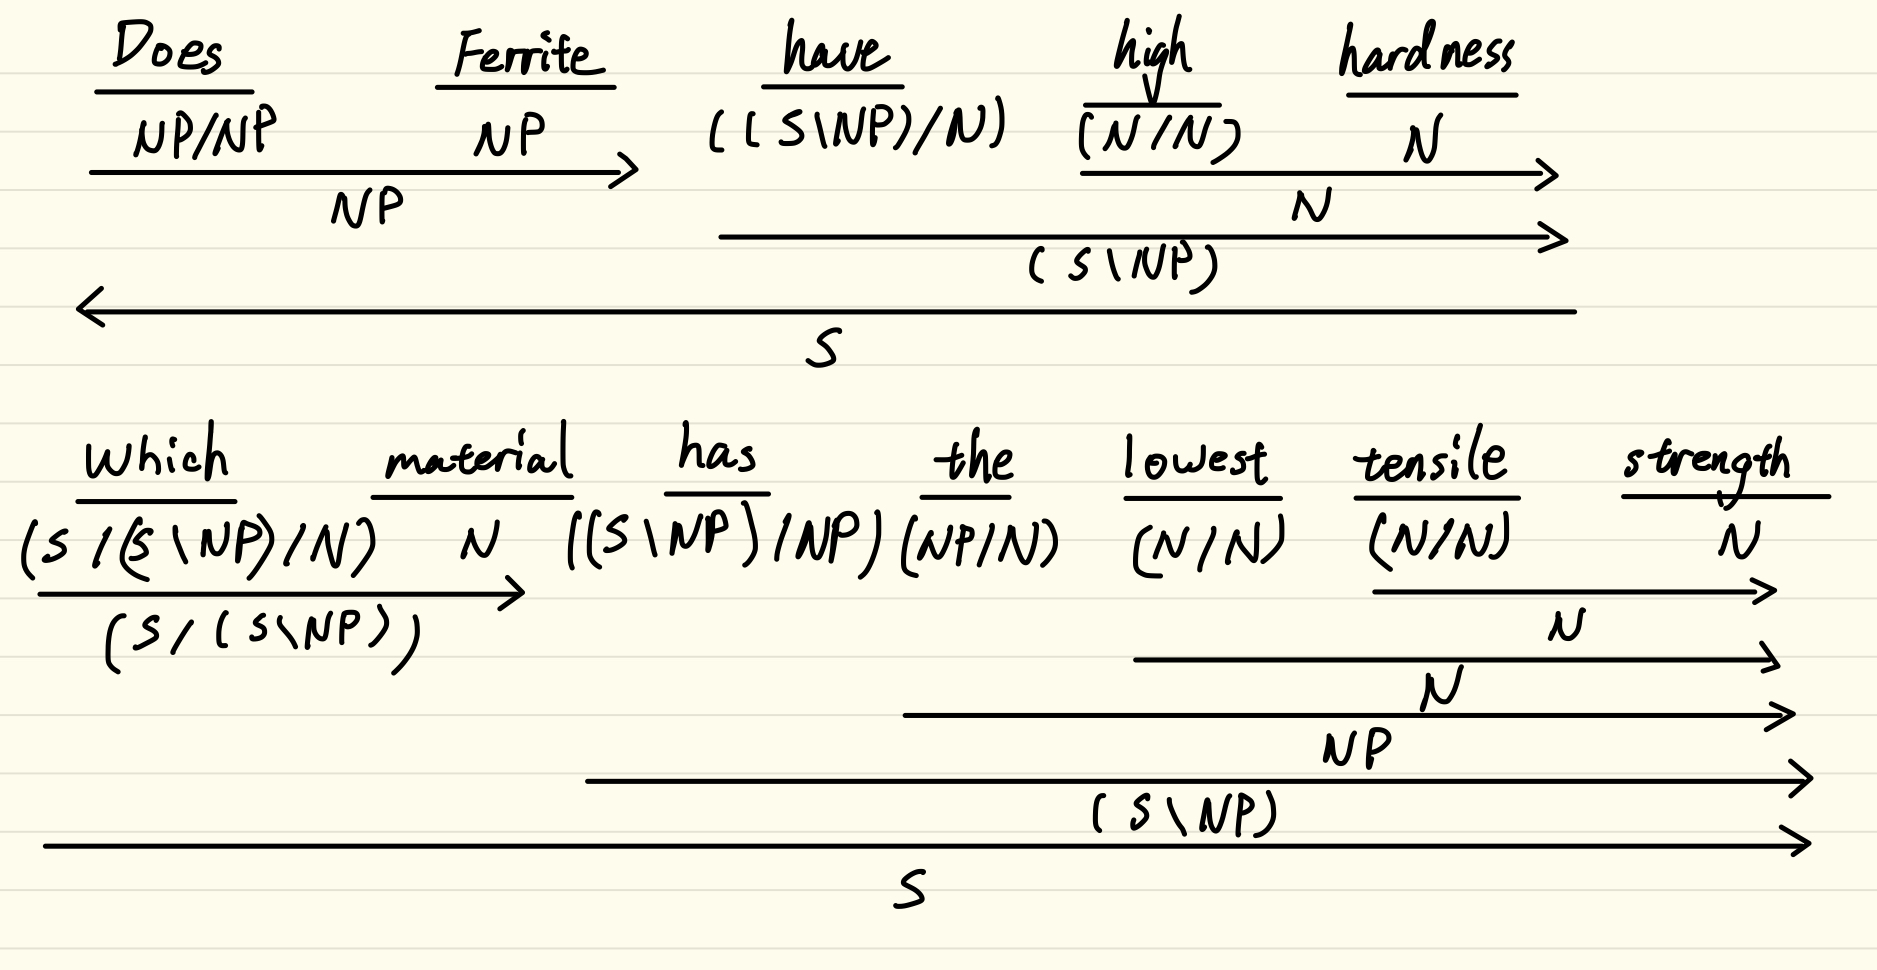
\includegraphics[scale=0.2]{figs/derTree2.jpg}
        \caption{derivation trees for questions}
        \label{label:derivation tree 2}
    \end{figure}
\end{enumerate}

\section{Ex5 CCG Syntactic Parser}
\label{sec: ex5}
\begin{enumerate}[1.]
    \item Implement a syntactic parser in NLTK for the grammar that you designed in the previous exercise.
    
    See the python file in appendix C.
    \item Print the derivation tree for the four sentences.
    \begin{figure}[ht]
        \centering
        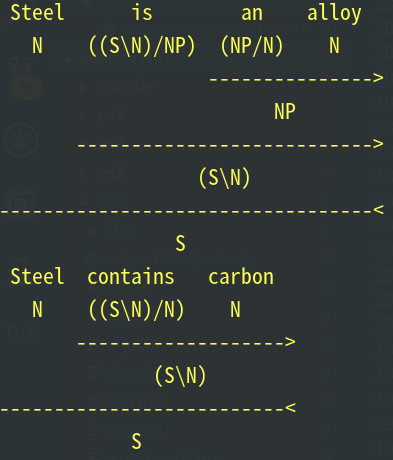
\includegraphics[scale=0.35]{figs/syntax-parse1.png}
        \caption{CCG syntactic parse for statements}
        \label{label:syntactic parse 1}
    \end{figure}
    \begin{figure}[ht]
        \centering
        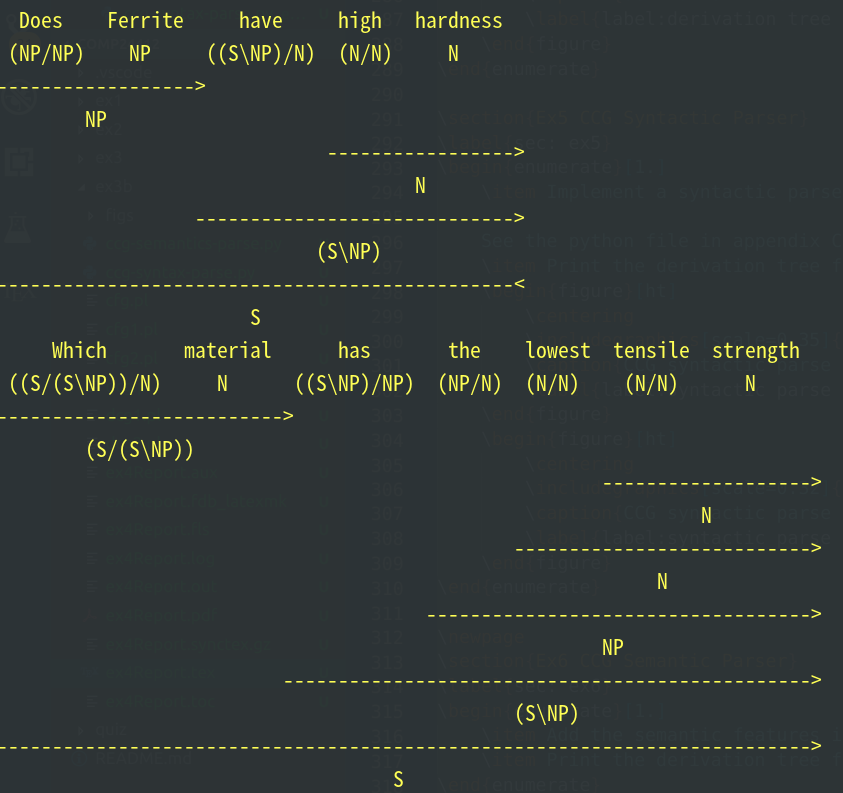
\includegraphics[scale=0.32]{figs/syntax-parse2.png}
        \caption{CCG syntactic parse for questions}
        \label{label:syntactic parse 2}
    \end{figure}
\end{enumerate}

\newpage
\section{Ex6 CCG Semantic Parser}
\label{sec: ex6}
\begin{enumerate}[1.]
    \item Add the semantic features into your grammar.
    
    See the python file with semantic features in appendix D.
    \item Print the derivation tree for the sentences in the corpus using the semantic features.
    \begin{figure}[ht]
        \centering
        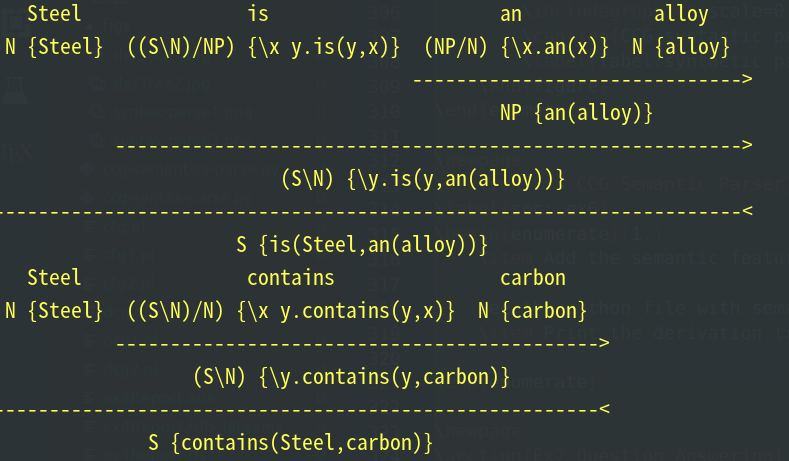
\includegraphics[scale=0.35]{figs/semantics-parse1.png}
        \caption{CCG semantics parse for statements}
        \label{label:semantics parse 1}
    \end{figure}
    \begin{figure}[ht]
        \centering
        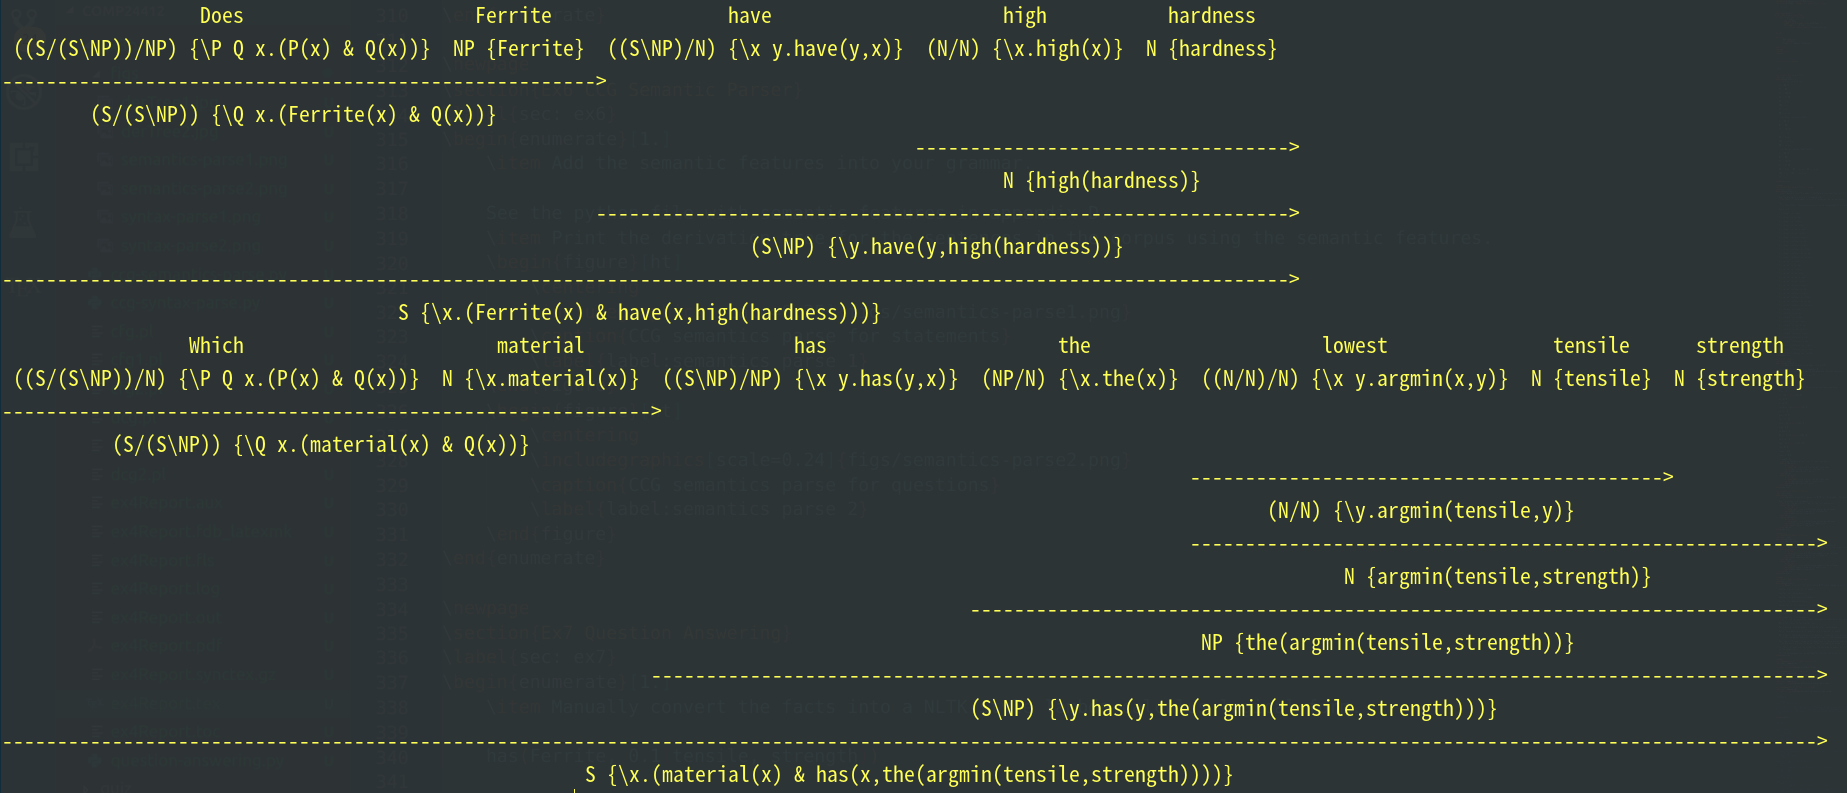
\includegraphics[scale=0.24]{figs/semantics-parse2.png}
        \caption{CCG semantics parse for questions}
        \label{label:semantics parse 2}
    \end{figure}
\end{enumerate}

\newpage
\section{Ex7 Question Answering}
\label{sec: ex7}
\begin{enumerate}[1.]
    \item Manually convert the facts into a NLTK-style lambda-calculus logical form.
    
    has(Ferrite, 0.1(tensile, strength))

    has(Ferrite, low(hardness))

    has(Perlite, 0.3(tensile, strength))

    has(Perlite, medium(hardness))

    has(Austenite, 0.4(tensile, strength))

    has(Austenite, medium(hardness))

    has(Cementite, 0.7(tensile, strength))

    has(Cementite, high(hardness))
    \item For the two questions, adapt the semantic features of your previous grammar to match the predicate form in the KB.
    
    I slightly adjust the semantics of the previous exercise so I can do the matchings:

    Match Ferrite(x) to Ferrite(Ferrite)

    Match has(x, high(hardness)) to has(Cementite, high(hardness))
    
    Match argmin(tensile, strength)) to 0.1(tensile, strength)
    
    Match has(x, argmin(tensile, strength)) to has(Ferrite, 0.1(tensile, strength))
    \item Run the parser and print the parse trees for the two questions.
    
    Parser output:

    $S \{\backslash x.(Ferrite(x) \& has(x,high(hardness)))\}$

    $S \{\backslash x.(material(x) \& has(x,argmin(tensile,strength)))\}$

    \begin{figure}[ht]
        \centering
        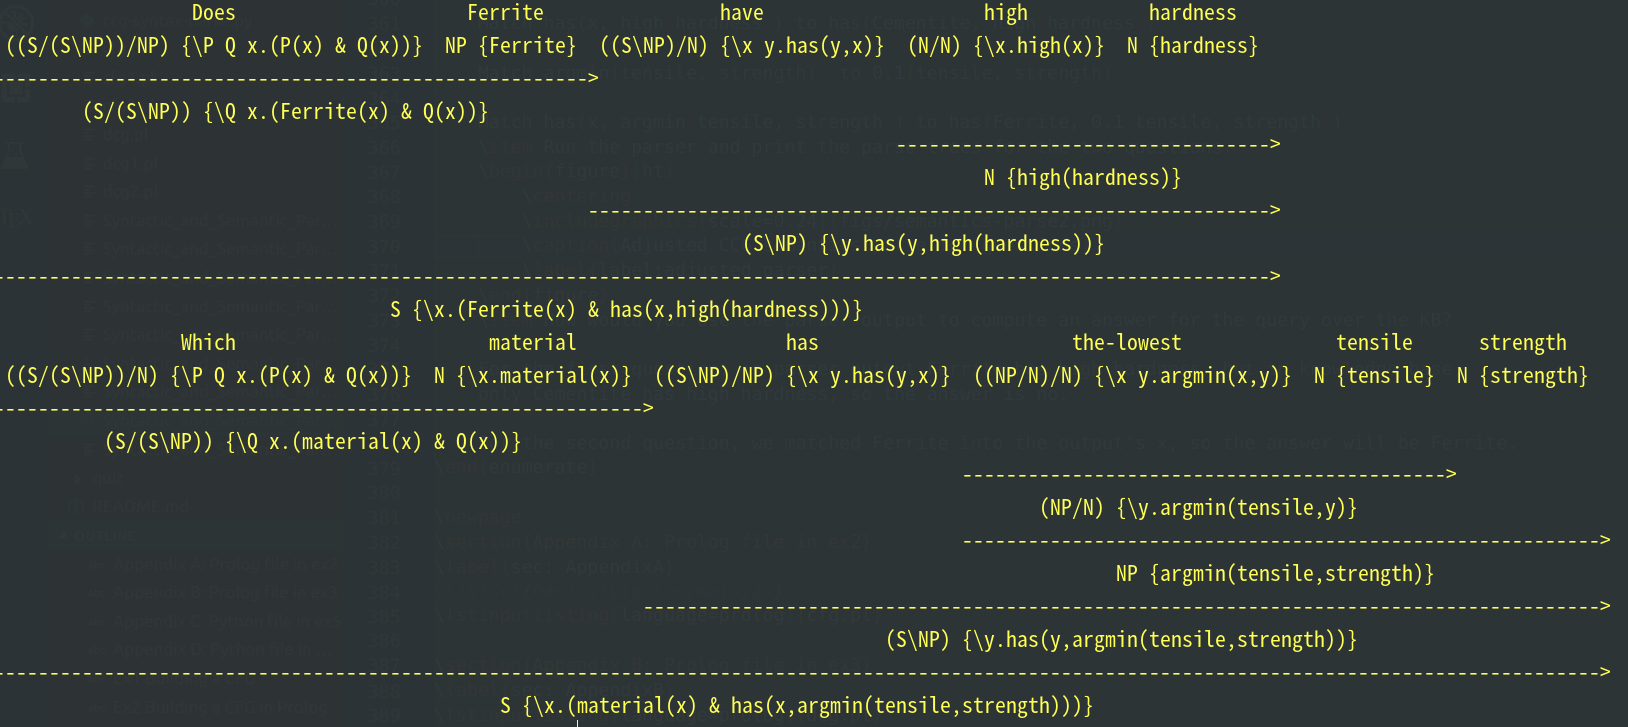
\includegraphics[scale=0.25]{figs/adjusted-semantics.png}
        \caption{Adjusted CCG semantics parse for questions}
        \label{label:adjusted parser}
    \end{figure}
    \item How would you use the parser output to compute an answer for the query over the KB?
    
    For the first question, in parser output x has high hardness, and in knowledge base, 
    only Cementite has high hardness, so we match x as Cementite, which is not agree with 
    Ferrite(x), so the answer is no.

    For the second question, we firstly search for argmin in the knowledge base, which is 0.1 among 
    0.1, 0.3, 0.4 and 0.7, and then we can match the "has" predicate, and here x is Ferrite, also, 
    Ferrite is a kind of material, so material(Ferrite) is true, so the answer of the query is Ferrite.
\end{enumerate}

\newpage
\section{Appendix A: Prolog file for ex2}
\label{sec: AppendixA}
%\lstset{basicstyle=\normalsize}
\lstinputlisting[language=prolog]{cfg.pl}

\section{Appendix B: Prolog file for ex3}
\label{sec: AppendixB}
\lstinputlisting[language=prolog]{dcg.pl}

\section{Appendix C: Python file for ex5}
\label{sec: AppendixC}
\lstinputlisting[language=python]{ccg-syntax-parse.py}

\section{Appendix D: Python file for ex6}
\label{sec: AppendixD}
\lstinputlisting[language=python]{ccg-semantics-parse.py}

\section{Appendix E: Python file for ex7}
\label{sec: AppendixD}
\lstinputlisting[language=python]{ccg-questions.py}

%-------------------------------------------------------------------------------
% REFERENCES
%-------------------------------------------------------------------------------
% \newpage
% \section*{References}

%[2]John W. Eaton, David Bateman, Sren Hauberg, Rik Wehbring (2015). GNU
%Octave version 4.0.0 manual: a high-level interactive language for numer-
%ical computations. Available: http://www.gnu.org/software/octave/doc/
%interpreter/. 
}
\end{document}

%-------------------------------------------------------------------------------
% SNIPPETS
%-------------------------------------------------------------------------------

%\begin{figure}[!ht]
%	\centering
%	\includegraphics[width=0.8\textwidth]{file_name}
%	\caption{}
%	\centering
%	\label{label:file_name}
%\end{figure}

%\begin{figure}[!ht]
%	\centering
%	\includegraphics[width=0.8\textwidth]{graph}
%	\caption{Blood pressure ranges and associated level of hypertension (American Heart Association, 2013).}
%	\centering
%	\label{label:graph}
%\end{figure}

%\begin{wrapfigure}{r}{0.30\textwidth}
%	\vspace{-40pt}
%	\begin{center}
%		\includegraphics[width=0.29\textwidth]{file_name}
%	\end{center}
%	\vspace{-20pt}
%	\caption{}
%	\label{label:file_name}
%\end{wrapfigure}

%\begin{wrapfigure}{r}{0.45\textwidth}
%	\begin{center}
%		\includegraphics[width=0.29\textwidth]{manometer}
%	\end{center}
%	\caption{Aneroid sphygmomanometer with stethoscope (Medicalexpo, 2012).}
%	\label{label:manometer}
%\end{wrapfigure}

%\begin{table}[!ht]\footnotesize
%	\centering
%	\begin{tabular}{cccccc}
%	\toprule
%	\multicolumn{2}{c} {Pearson's correlation test} & \multicolumn{4}{c} {Independent t-test} \\
%	\midrule	
%	\multicolumn{2}{c} {Gender} & \multicolumn{2}{c} {Activity level} & \multicolumn{2}{c} {Gender} \\
%	\midrule
%	Males & Females & 1st level & 6th level & Males & Females \\
%	\midrule
%	\multicolumn{2}{c} {BMI vs. SP} & \multicolumn{2}{c} {Systolic pressure} & \multicolumn{2}{c} {Systolic Pressure} \\
%	\multicolumn{2}{c} {BMI vs. DP} & \multicolumn{2}{c} {Diastolic pressure} & \multicolumn{2}{c} {Diastolic pressure} \\
%	\multicolumn{2}{c} {BMI vs. MAP} & \multicolumn{2}{c} {MAP} & \multicolumn{2}{c} {MAP} \\
%	\multicolumn{2}{c} {W:H ratio vs. SP} & \multicolumn{2}{c} {BMI} & \multicolumn{2}{c} {BMI} \\
%	\multicolumn{2}{c} {W:H ratio vs. DP} & \multicolumn{2}{c} {W:H ratio} & \multicolumn{2}{c} {W:H ratio} \\
%	\multicolumn{2}{c} {W:H ratio vs. MAP} & \multicolumn{2}{c} {\% Body fat} & \multicolumn{2}{c} {\% Body fat} \\
%	\multicolumn{2}{c} {} & \multicolumn{2}{c} {Height} & \multicolumn{2}{c} {Height} \\
%	\multicolumn{2}{c} {} & \multicolumn{2}{c} {Weight} & \multicolumn{2}{c} {Weight} \\
%	\multicolumn{2}{c} {} & \multicolumn{2}{c} {Heart rate} & \multicolumn{2}{c} {Heart rate} \\
%	\bottomrule
%	\end{tabular}
%	\caption{Parameters that were analysed and related statistical test performed for current study. BMI - body mass index; SP - systolic pressure; DP - diastolic pressure; MAP - mean arterial pressure; W:H ratio - waist to hip ratio.}
%	\label{label:tests}
%\end{table}%\documentclass{article}
%\usepackage[utf8]{inputenc}

%\title{Weekly Report template}
%\author{gandhalijuvekar }
%\date{January 2019}

%\begin{document}

%\maketitle

%\section{Introduction}

%\end{document}